
A partir de lo programado en \textit{Unity PRO} utilizado para obtener los primeros registros, se realizaron las modificaciones necesarias donde se eliminaron y agregaron variables de la lista de direcciones (Tabla {\ref{tab:direc} en Anexo \ref{Anexo1}). El mapa de memoria del proyecto se divide según la figura \ref{fig:memoria}.
	
\begin{figure}[h!]
	\centering
	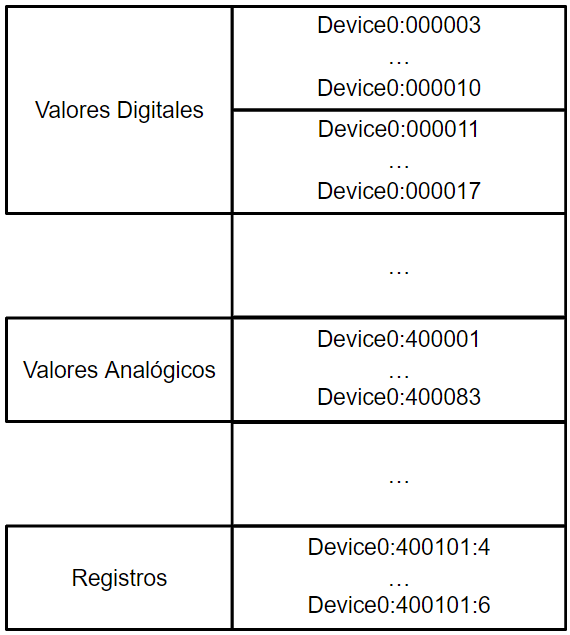
\includegraphics[scale=0.6]{memoria.png}
	\captionof{figure}{Mapa de memoria}
	\label{fig:memoria}
\end{figure}


\subsection{Adquisición de datos}
En el objetivo se propuso que el sistema sea capaz de controlar presión o caudal. Para lograr lo estipulado, como en cualquier sistema de control, es necesario conocer las plantas con las que se trabajará, dónde se distinguen en el banco de pruebas tres sistemas distintos:
\begin{itemize}
	\item PIT01: Presión medida a la salida de la bomba.
	\item PIT02: Presión medida luego de la columna de derivación.
	\item FT01: Caudal que pasa por PIT02.
\end{itemize}

Para realizar las estimaciones de los sistemas se utilizó el protocolo OPC en conjunto con \textit{Matlab}. Por medio de OFS, se procedió a crear y configurar un servidor(Figura \ref{fig:opc1}).

\begin{figure}[h!]
	\centering
	\subfigure[]{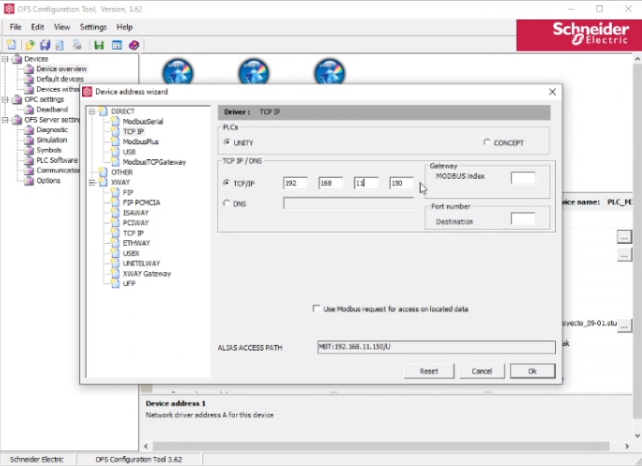
\includegraphics[scale=0.6]{ofs1.png}}
	\subfigure[]{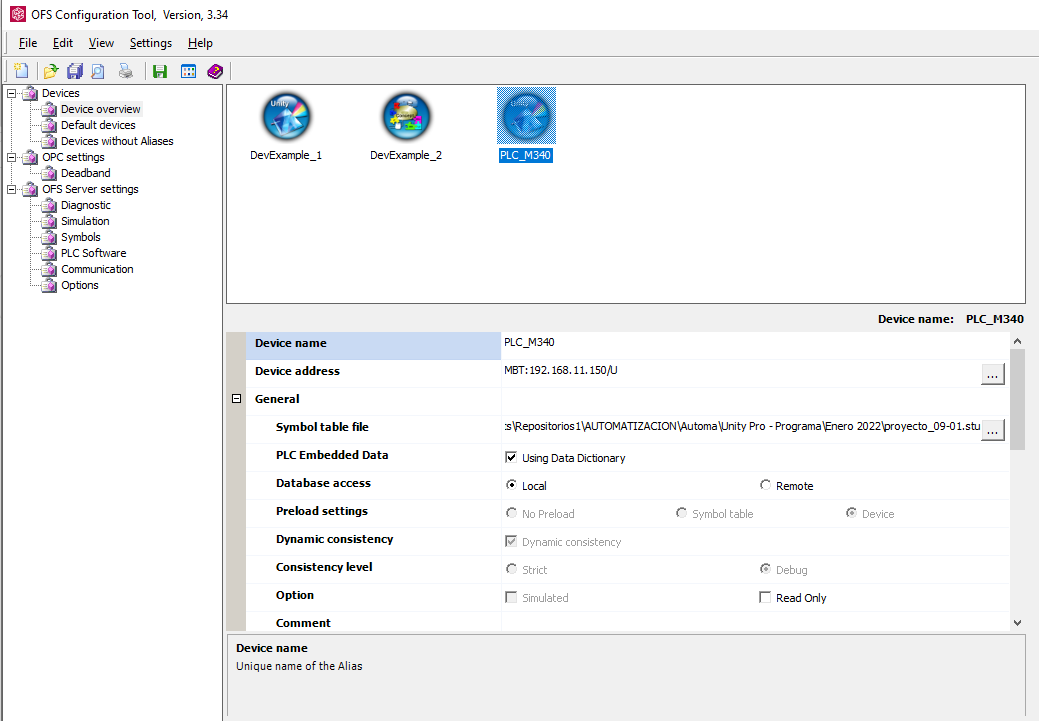
\includegraphics[scale=0.5]{ofs2.png}}
	\caption{Configuración OFS} \label{fig:opc1}
\end{figure}


Una vez configurado, se abre el programa \textit{OPC Factory Server} y se da inicio al servidor (Figura \ref{fig:opc2}.a). Para observar si la comunicación se estableció de forma correcta, se utilizó el programa \textit{OFS Client} (Figura \ref{fig:opc2}.b).

\begin{figure}[h!]
	\centering
	\subfigure[OPC Factory Server]{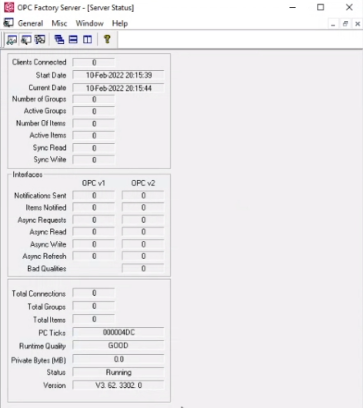
\includegraphics[scale=0.7]{ofs3.png}}
	\subfigure[OFS Client]{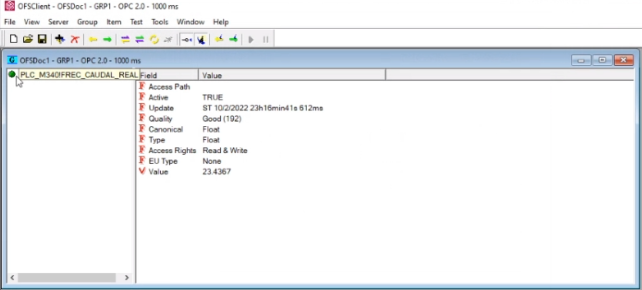
\includegraphics[scale=0.6]{ofs4.png}}
	\caption{Conexión servidor OPC} \label{fig:opc2}
\end{figure}

Una vez corroborada la comunicación con el servidor OPC, se procedió a crear un cliente OPC en \textit{Simulink} (perteneciente a \textit{Matlab}) para adquirir y guardar las variables necesarias. 


\subsubsection{Uso de Matlab}
En el entorno \textit{Simulink} se procedió a configurar un bloque de cliente OPC con la dirección IP donde se encuentra el servidor previamente creado. Luego, para leer las variables necesarias se creó un bloque de lectura OPC (Figura \ref{fig:opcsimu}.a) y con un bloque \textit{Scope}, se activó la opción para que se guarden los vectores de las variables a estudiar (Figura \ref{fig:opcsimu}.b) para luego ser guardados en un archivo \textit{.csv} .





\begin{figure}[h!]
	\centering
	\subfigure[]{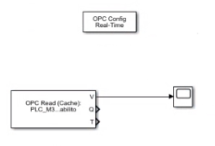
\includegraphics[width=60mm]{ofs5.png}}
	\subfigure[]{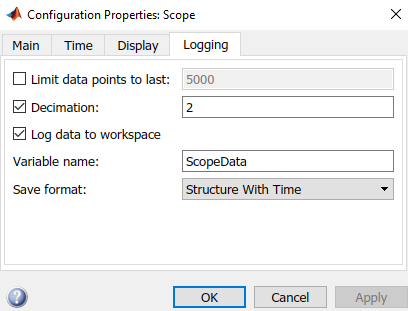
\includegraphics[width=60mm]{ofs6.png}}
	\caption{Cliente OPC en Simulink} \label{fig:opcsimu}
\end{figure}

Se configuró el bloque OPC Read (Figura \ref{fig:muestr}) con una frecuencia de muestreo de 50 ms ya que el valor es 10 veces más rápido que el polo del sistema más rápido.
\begin{figure}[htb]
	\centering
	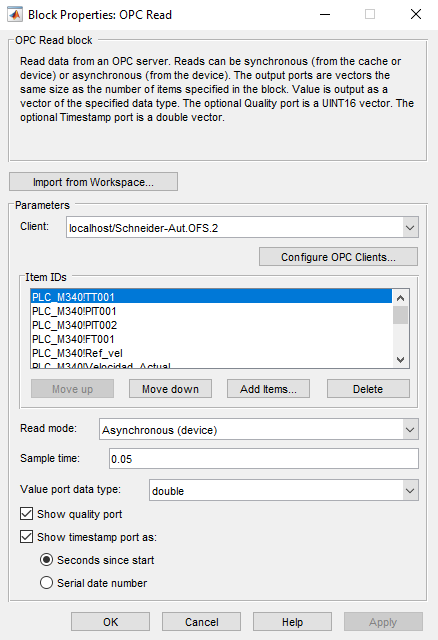
\includegraphics[width=0.6\linewidth]{frecmuestreo.png}
	\captionof{figure}{Configuración de frecuencia de muestreo}
	\label{fig:muestr}
\end{figure}





\subsubsection{Estimación de la planta}
Para realizar la estimación de las plantas se utilizó el Método de Strejc con retardo (Figura \ref{fig:norden})\cite{pomares2011sistemas}.
Este método se emplea para la identificación de sistemas de polos múltiples,
mediante los parámetros \textit{Tu} y \textit{Ta} obtenidos sobre la respuesta del sistema.
Tras obtener el valor de los parámetros, se determina la multiplicidad del polo. 
\begin{figure}[h!]
	\centering
	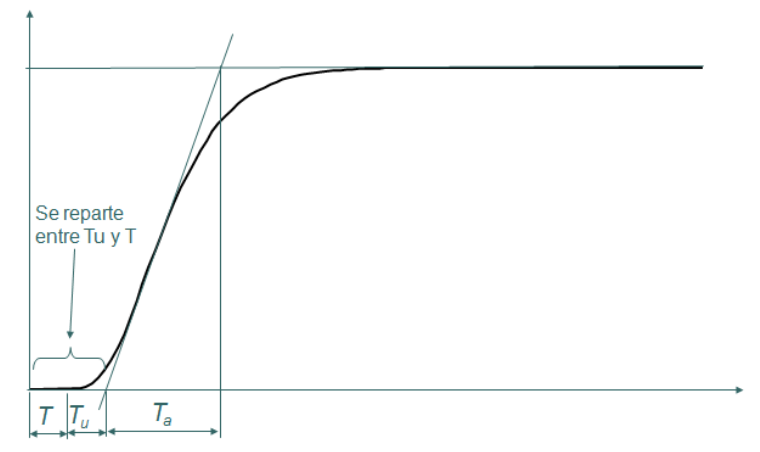
\includegraphics[width=0.9\linewidth]{norden.png}
	\captionof{figure}{Parámetros de Strejc con retardo}
	\label{fig:norden}
\end{figure}

La función de transferencia general para un sistema de polos múltiples es:
\begin{equation}
	G(s)\;=\;\frac K{(1\;+\;\tau\;.\;s)^n}\;.\;e^{-T.s}
\end{equation}
Dónde:
\begin{itemize}
	\item K:  Ganancia del sistema $K = \frac{\triangle y}{\triangle u}$
	\item $\tau$: constante de tiempo
	\item T= Retardo
\end{itemize}

Para obtener la función de transferencia se realizó un programa en \textit{Matlab} que dió como resultado los siguientes sistemas:
\begin{itemize}
	\item Planta de presión PIT01:
	\begin{equation}
	 G(s)\;=\;\frac {0,135}{(1\;+\;1,3783\;.\;s)^3}\;.\;e^{-1,2.s}
	\end{equation}
	\item Planta de presión PIT02: 	
	\begin{equation}
		G(s)\;=\;\frac {0,125}{(1\;+\;1,054\;.\;s)^3}\;.\;e^{-s}
	\end{equation}
	\item Planta de caudal FT01:
		\begin{equation}
		G(s)\;=\;\frac {0,003784}{(1\;+\;0,7027\;.\;s)^3}\;.\;e^{-s}
	\end{equation}
\end{itemize}

\paragraph{Comparación numérica- real}
En las siguientes imágenes (Figura \ref{fig:PIT01} ,\ref{fig:PIT02} y \ref{fig:FT01}) se observa la gráfica de cada planta estimada comparada con los datos obtenidos en las mediciones.
\begin{comment}
$C:\Users\glori\Desktop\DANIELA\VISUAL_DANI\Automa\MATLAB\Prueba_PLANTA\Imaagenes Calculo Plantas\FIT001
Strenj_RESPUESTA.png$
\end{comment}

Cabe destacar que las plantas fueron calculadas para los rangos medios que normalmente se utilizará dado que los sistemas de presión no presentan una ganancia estática constante.

Se puede observar que los sistemas de tercer orden se adaptan bien a los datos obtenidos durante las pruebas.
\begin{comment}
no borrar opr las dudas que quisimos poner esto
 
 dónde el motor no era esforzado a calentarse ni la bomba era sobreexigida

escalones ubicados en la parte central del rango útil estipulado .

 además obtener un control apropiado al sistema: algo no muy rapido ni muy lento
\end{comment}


\begin{figure}[h!]
	\centering
	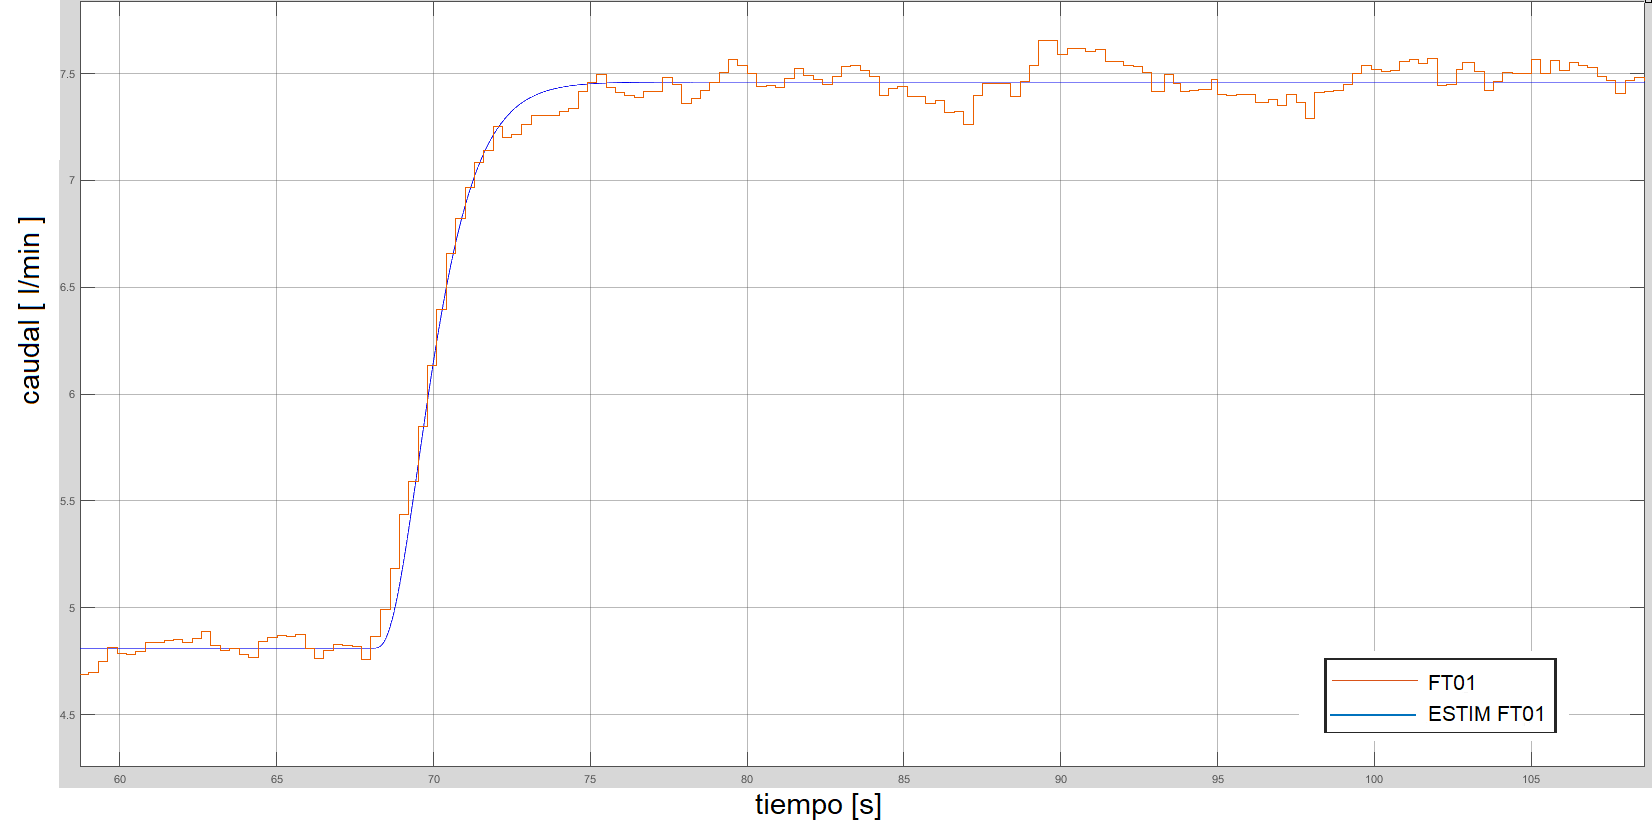
\includegraphics[width=0.8\linewidth]{Strenj_RESPUESTA.png}
	\captionof{figure}{Comparación de la planta estimada y los valores obtenidos para FT01}
	\label{fig:FT01}
\end{figure}
\begin{figure}[h!]
	\centering
	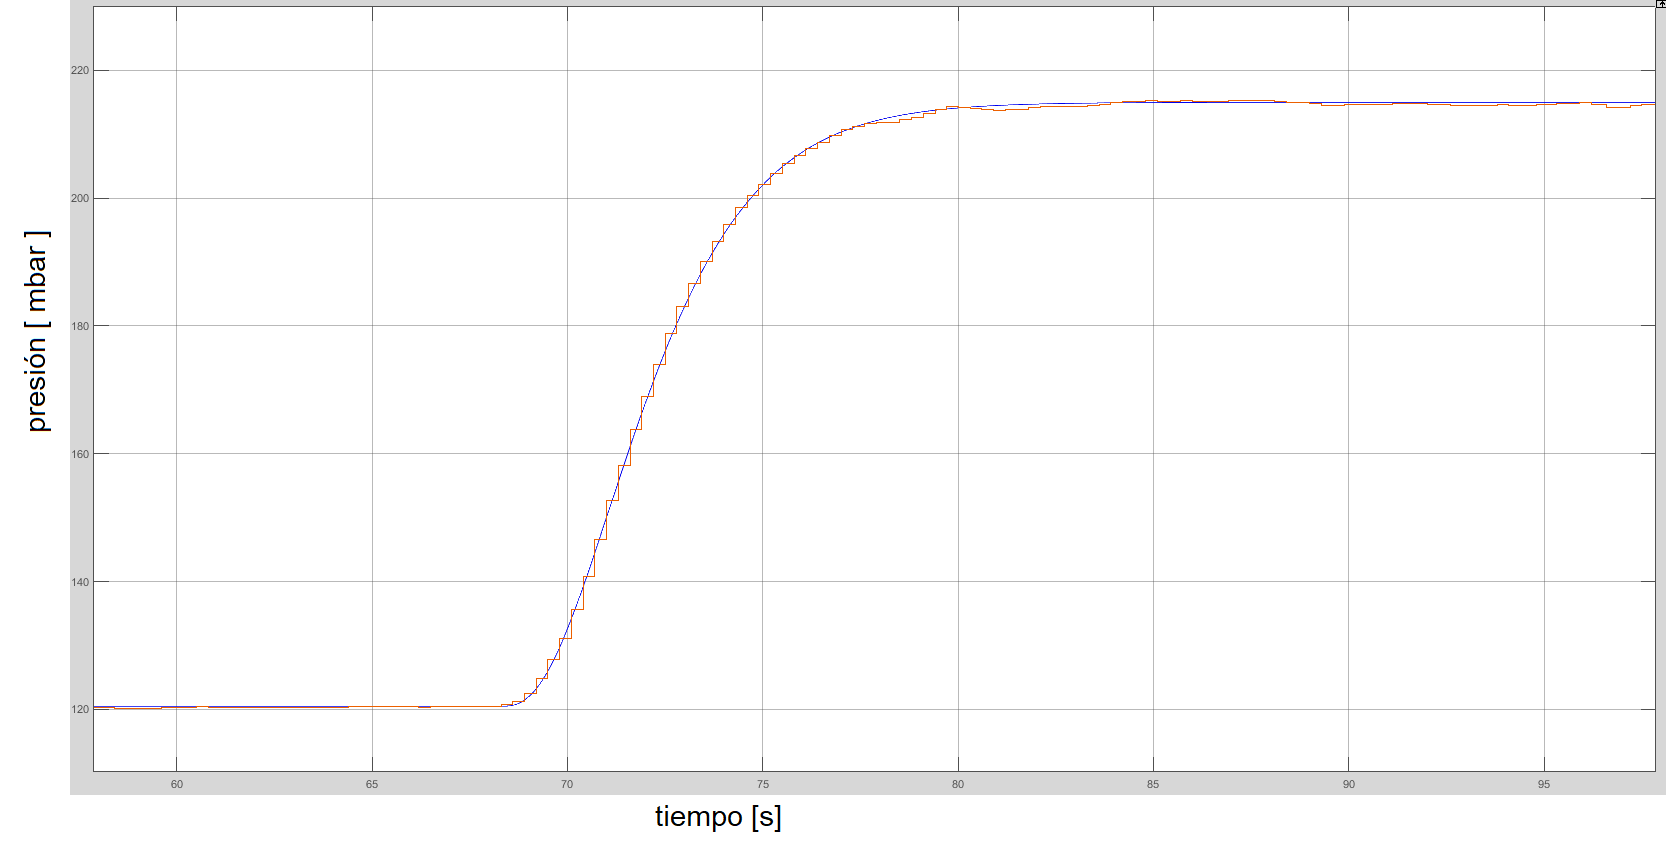
\includegraphics[width=0.8\linewidth]{Strenj_RESPUESTA1.png}
	\captionof{figure}{Comparación de la planta estimada y los valores obtenidos para PIT01}
	\label{fig:PIT01}
\end{figure}




\begin{figure}[h!]
	\centering
	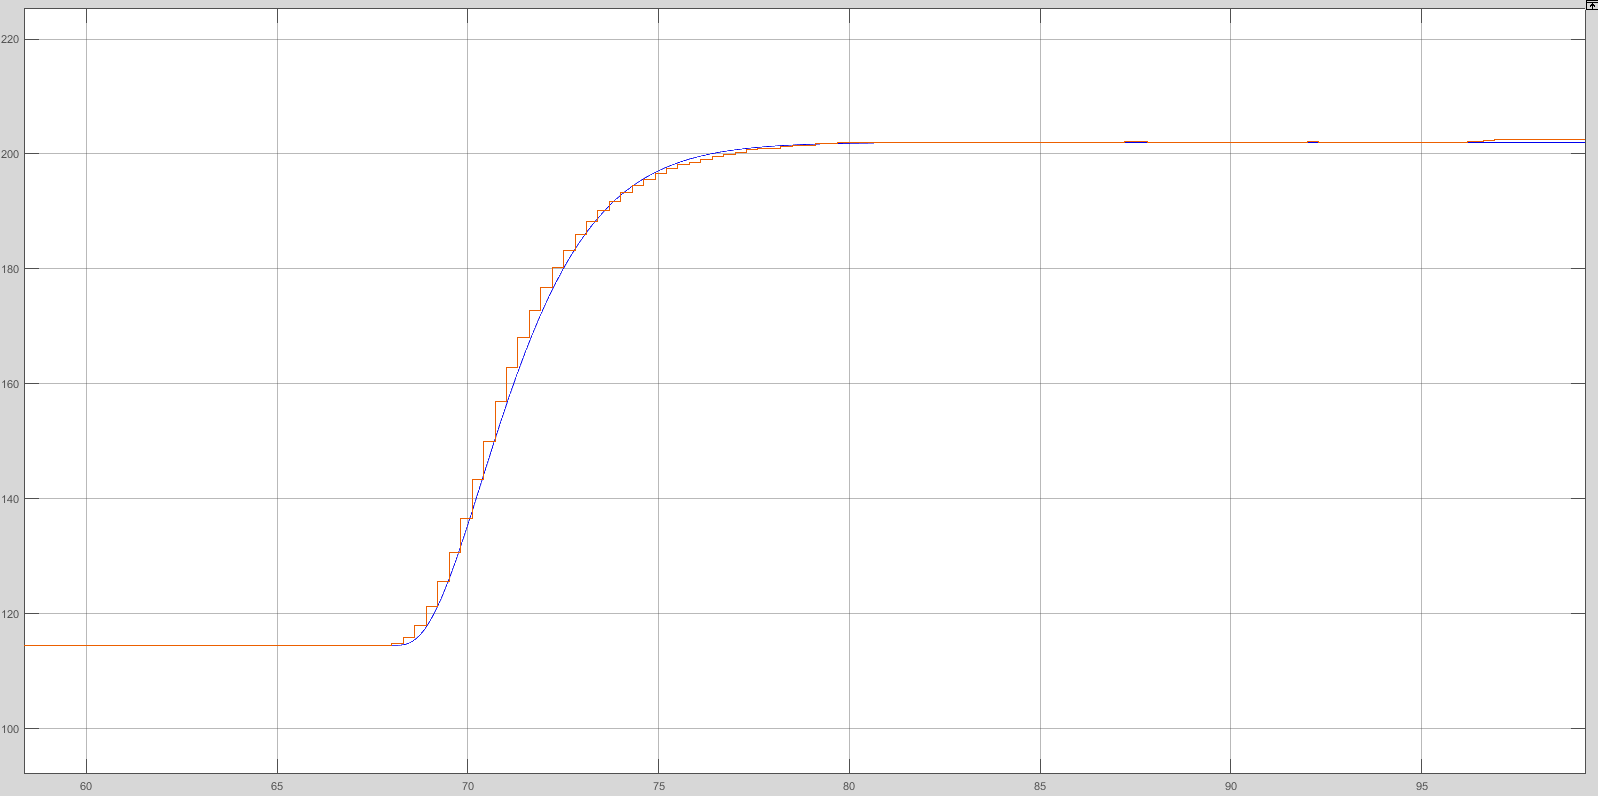
\includegraphics[width=0.8\linewidth]{Strenj_respuesta2.png}
	\captionof{figure}{Comparación de la planta estimada y los valores obtenidos para PIT02}
	\label{fig:PIT02}
\end{figure}





\clearpage
\subsubsection{Cálculo del controlador PID}
El controlador PID de cada planta se calculó con \textit{Tune PID controllers} (Figura \ref{fig:PIDcontr}), dónde se buscó que la respuesta al escalón en estado estacionario sea nula y además sea capaz de mitigar los cambios producidos por la ganancia variable en los sistemas de presión ocasionados por la característica de la bomba. 

Se realizaron pruebas con diversos PID para observar la respuesta a cada sistema, en las figuras \ref{fig:FT1} , \ref{fig:PIT1} y \ref{fig:PIT2} se comparan dos PI para cada planta, para elegir los parámetros del controlador se buscó que las respuestas lleguen al valor de referencia de una forma suave y con el mínimo sobrepaso.

Los valores obtenidos de la aplicación perteneciente a \textit{Matlab} se muestran en la tabla \ref{tab:pid}, los cuales se ingresaron en los bloques de \textit{UnityPro} con las respectivas modificaciones numéricas según lo establecido por el software. Los valores mostrados en dicha tabla serán usados al momento de restablecer la configuración de los PI en la ventana de configuración del sistema SCADA.
\begin{figure}[h!]
	\centering
	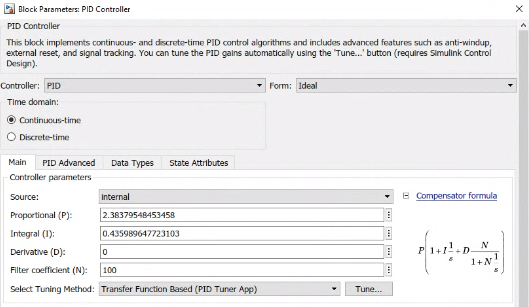
\includegraphics[scale=0.7]{pidmatlab.png}
	\captionof{figure}{PID Controller}
	\label{fig:PIDcontr}
\end{figure}



\begin{table}[h]
	\centering
	\begin{tabular}{|l|l|l|l|}
		\hline
		& PIT01 & PIT02 & FT01 \\ \hline
		$K_p$ & 3,05 & 5,453 & 104,3 \\ \hline
		$K_i$ & 0,396 & 0,348 & 0,719 \\ \hline
		$K_d$ & 0 & 0 & 0 \\ \hline
		N & 1000 & 1000 & 1000 \\ \hline
	\end{tabular}
	\captionof{table}{Valores de los PID}
	\label{tab:pid}
\end{table}

\begin{comment}
	C:\Users\glori\Desktop\DANIELA\VISUAL_DANI\Automa\MATLAB\22-05\Comparacion PID y PLANTAS\FT01
	Respuesta_Strenj
\end{comment}






\begin{figure}[h!]
	\centering
	\subfigure[]{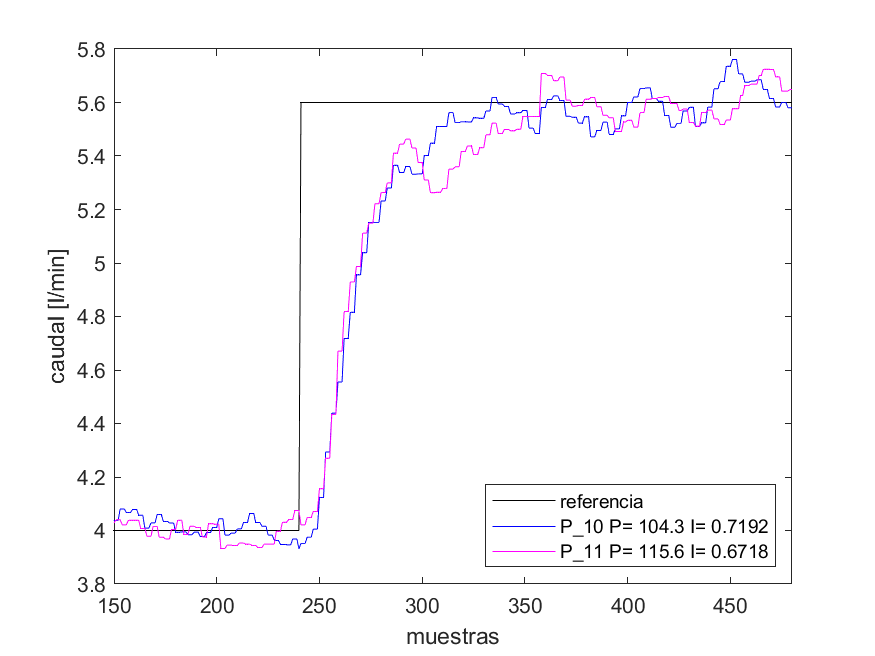
\includegraphics[width=80mm]{FT1b.png}}
\hspace{-4mm}
	\subfigure[]{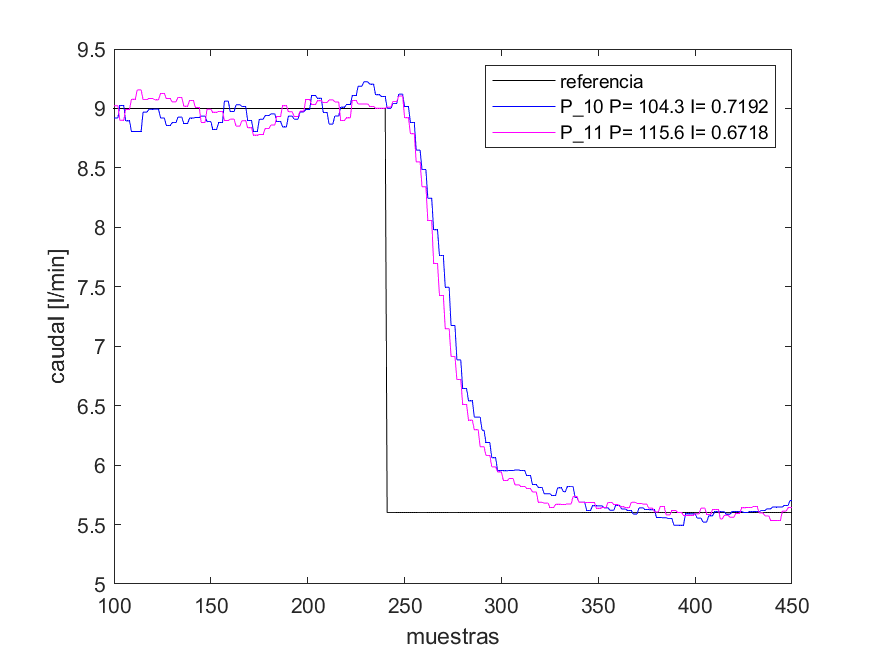
\includegraphics[width=80mm]{FT1c.png}}
	\caption{Comparación PI para FT01} \label{fig:FT1}
\end{figure}

\begin{figure}[h!]
	\centering
	\subfigure[]{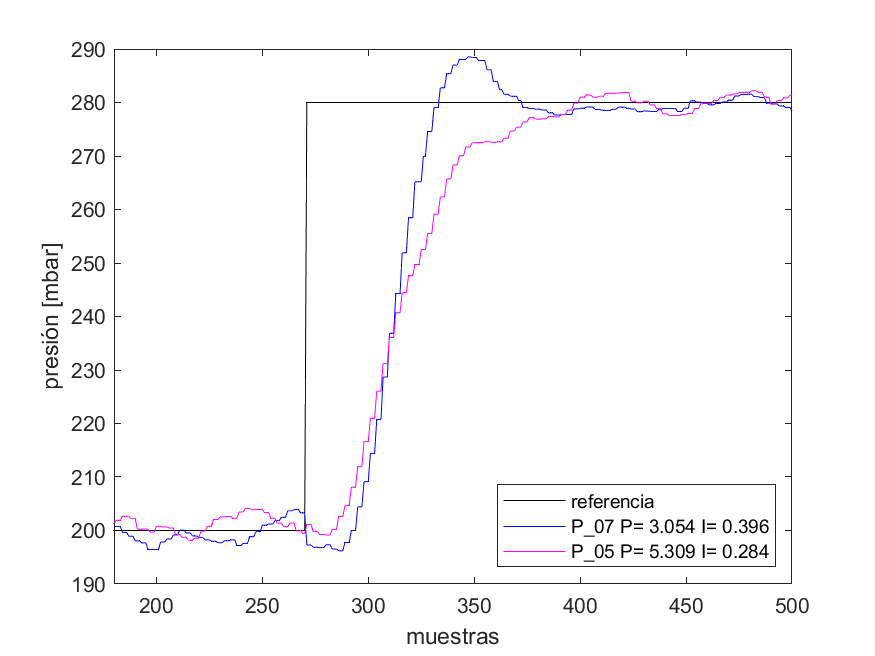
\includegraphics[width=80mm]{PIT1b.png}}
\hspace{-4mm}
	\subfigure[]{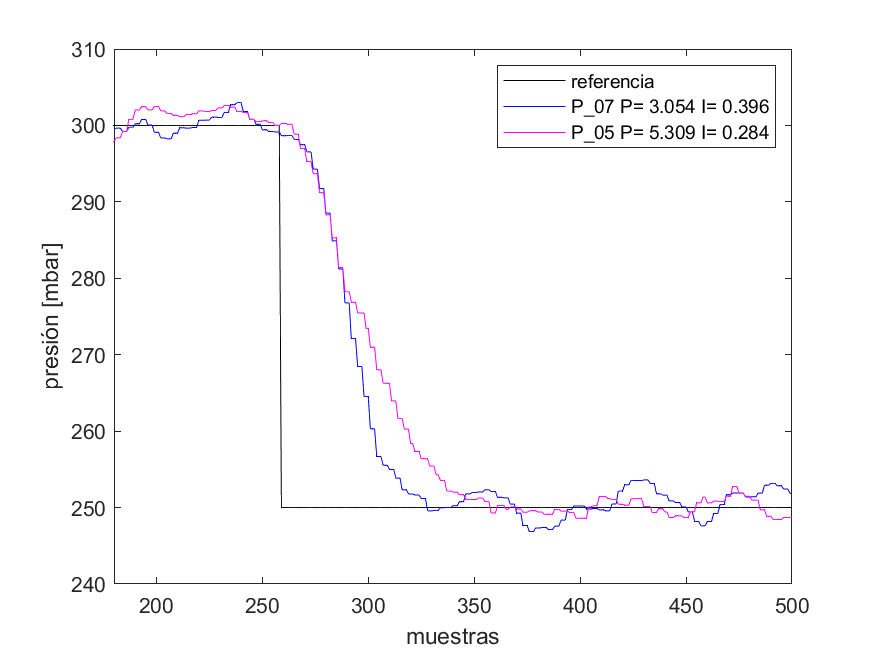
\includegraphics[width=80mm]{PIT1c.png}}
	\caption{Comparación PI para PIT01} \label{fig:PIT1}
\end{figure}

\begin{figure}[h!]
	\centering
	\subfigure[]{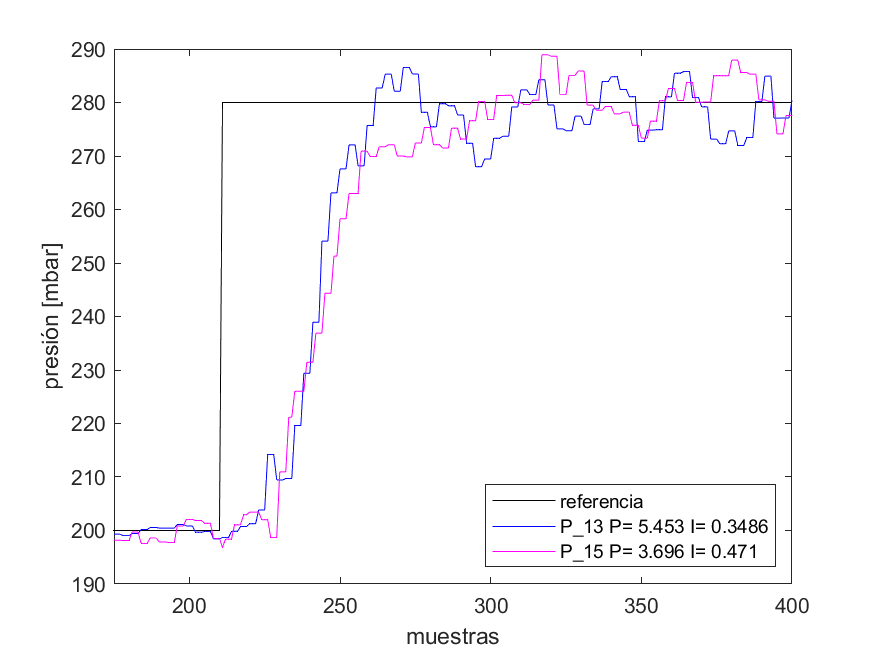
\includegraphics[width=80mm]{PIT2a.png}}
	\hspace{-4mm}
	\subfigure[]{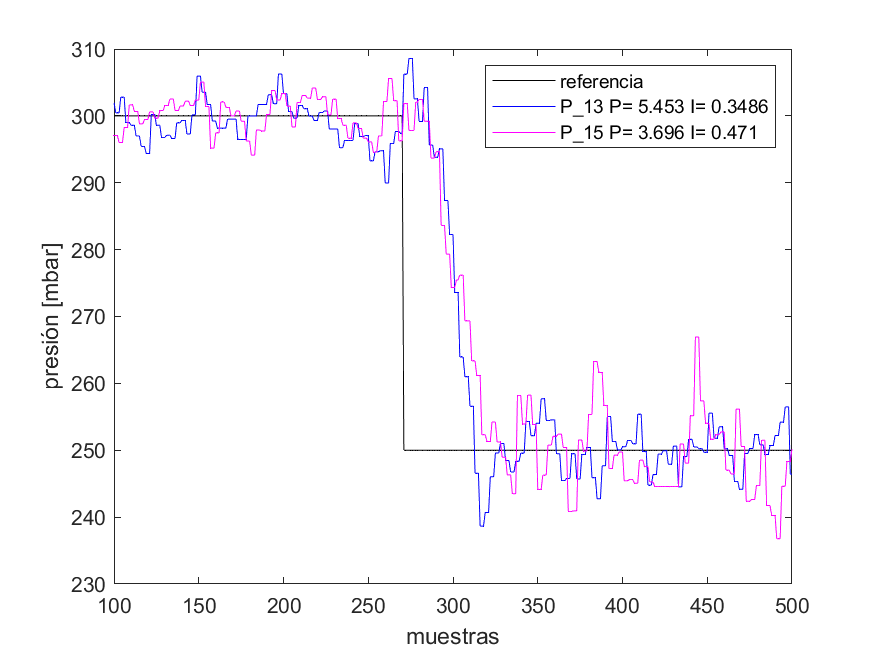
\includegraphics[width=80mm]{PIT2b.png}}
	\caption{Comparación PI para PIT02} \label{fig:PIT2}
\end{figure}

\clearpage
\subsubsection{Pruebas de control}

Para corroborar que cada sistema funcione correctamente ante perturbaciones se abrió y cerró las válvulas del banco de pruebas mostradas en el diagrama P\&ID de la figura \ref{fig:diag2} que causan distintas alteraciones a la presión y caudal.
\begin{figure}[h!]
	\centering
	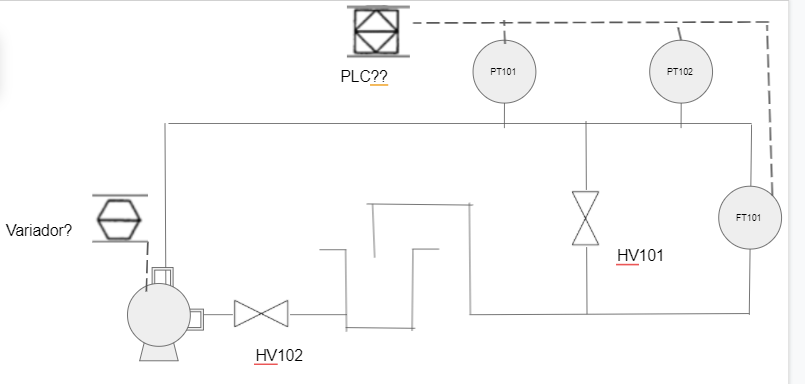
\includegraphics[width=1\linewidth]{diag.png}
	\captionof{figure}{Diagrama p\&id}
	\label{fig:diag2}
\end{figure}


\paragraph{Perturbación al control con PIT02}
En la figura \ref{fig:per2} se observa que el valor de referencia inicial es de 250 mbar; aproximadamente a los 15 segundos de comenzar la prueba se abrió totalmente la válvula de derivación FV01, y disminuyó la presión notablemente. Al pasar el tiempo y una vez que la presión llegó nuevamente a su punto de trabajo, se incrementó su valor a 300 mbar, se puede apreciar en el gráfico que la presión se acerca pero no llega a la referencia debido a que el motor, ya en su máxima frecuencia de trabajo, no logra elevar más la presión. Luego, a los 100 segundos de empezar la prueba, se cerró la válvula de derivación completamente y se observa como la presión se incrementó y disminuyó hasta que llegó al punto de referencia.
\begin{figure}[h!]
	\centering
	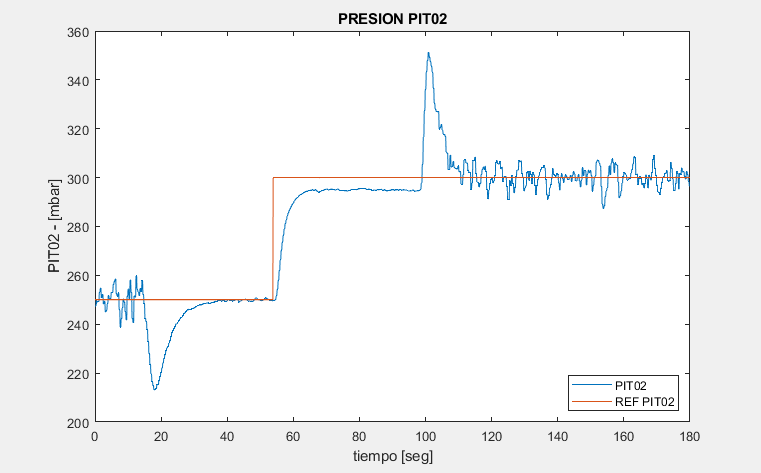
\includegraphics[width=0.9\linewidth]{Per2.png}
	\captionof{figure}{Perturbación al control con PIT02}
	\label{fig:per2}
\end{figure}

\paragraph{Perturbación al control de FT01}
Para la prueba de control con FT01 (Figura \ref{fig:per1}) como variable de proceso, se fijó el valor de referencia en 3,5 L/min a los 20 segundos se empezar la prueba. Luego, se abrió la válvula FV01 completamente y se observó la disminución del caudal, la acción de control elevó las revoluciones del motor hasta llegar a su punto de trabajo. Aproximadamente a los 125 segundos se configuró el valor de referencia en 2 L/min y se cerró la válvula FV01, esto provocó que todo el caudal circule por FT01. La acción de control disminuyó las revoluciones del motor hasta llegar al valor de caudal de referencia.

\begin{figure}[h!]
	\centering
	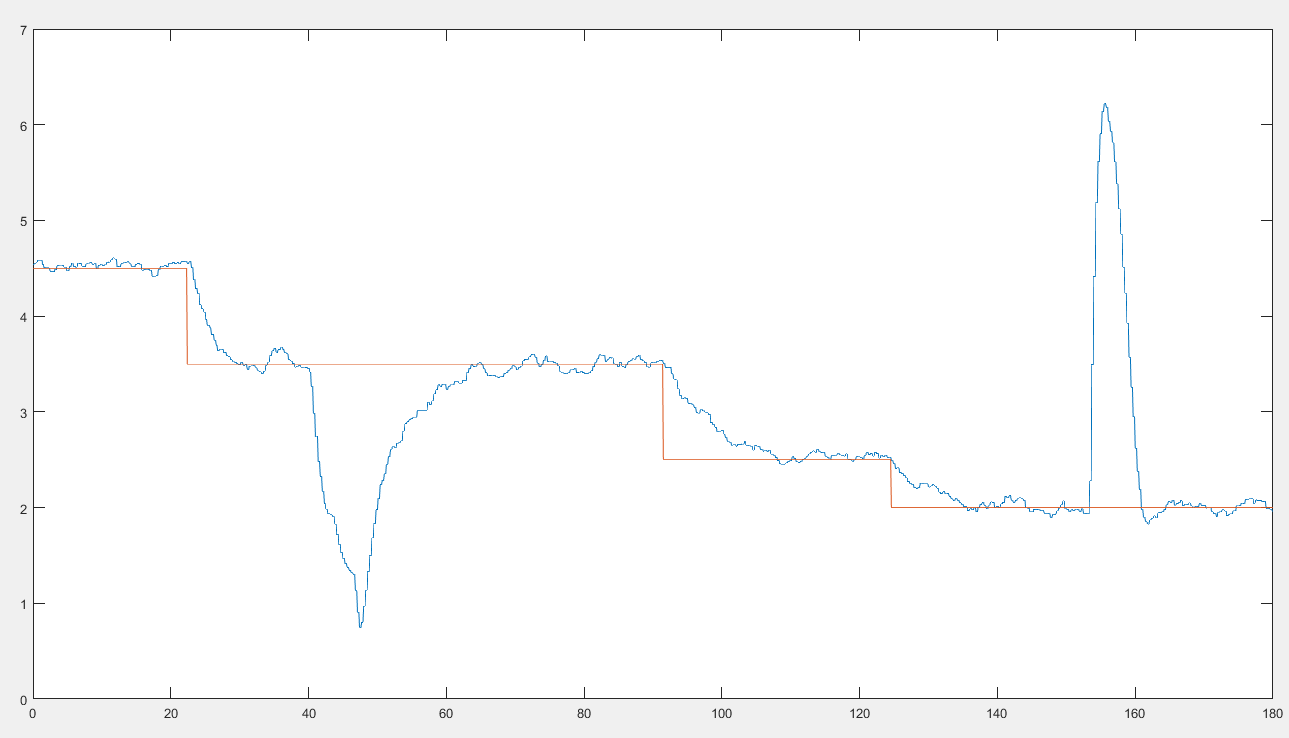
\includegraphics[width=0.9\linewidth]{PerF1.png}
	\captionof{figure}{Perturbación al control con FT01}
	\label{fig:per1}
\end{figure}


\subsubsection{Valores extremos/críticos de estudio}
En estas sub-secciones se muestra valores máximos de presión y caudal alcanzados en el banco de pruebas y el valor mínimo de presión a velocidad baja del motor.

\paragraph{Máxima presión}

Para esta prueba se llevó al motor a su máxima frecuencia (60Hz) de trabajo, se dejó la válvula FV03 totalmente abierta y se cerraron las válvulas FV01 y FV02 (Figura  \ref{fig:diag}). Esto provocó que la bomba llegue a su máxima presión que se obtiene al momento en que el caudal que circula por PIT01 se hace muy próximo a cero.\\
\textbf{\textit{Máxima presión:}} 938 mbar.
\begin{figure}[h!]
	\centering
	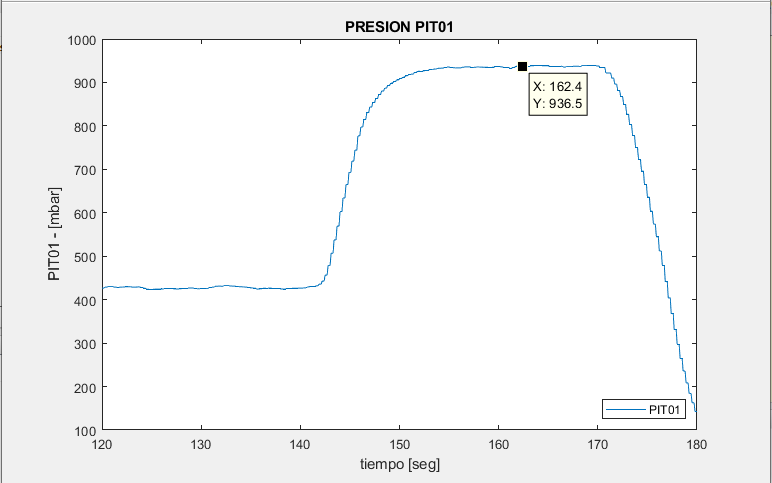
\includegraphics[width=0.9\linewidth]{Presion_Max.png}
	\captionof{figure}{Máxima presión}
	\label{fig:PMAX}
\end{figure}

\paragraph{Mínima presión}
Para obtener el valor de mínima presión de trabajo se configuró el VSD a 20 Hz y se abrieron todas las válvulas (Figura  \ref{fig:diag}), ésto generó que la bomba impulse el caudal con el menor esfuerzo. \\
\textbf{\textit{Mínima presión:}} 65,43 mbar
\begin{figure}[h!]
	\centering
	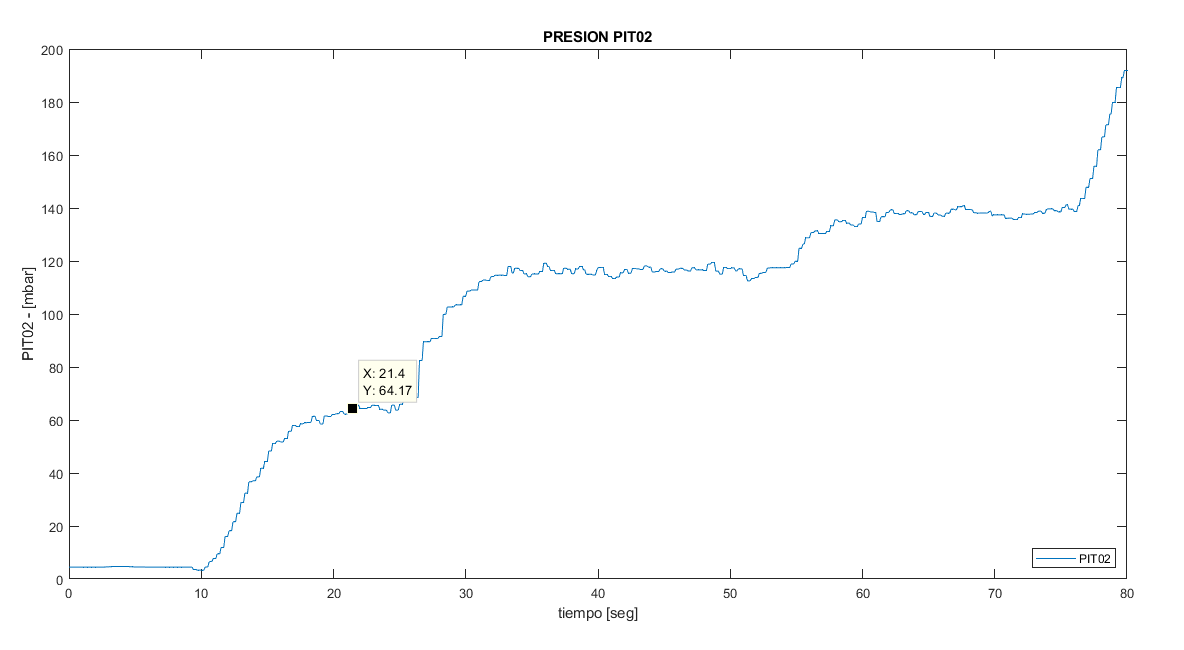
\includegraphics[width=0.9\linewidth]{Presion_Min.png}
	\captionof{figure}{Mínima presión}
	\label{fig:Pmin}
\end{figure}

\paragraph{Máximo caudal}
Para obtener el valor de caudal máximo se llevó al motor a su máxima frecuencia (60 Hz), se abrió completamente la válvula FV03 y FV02, y se cerró la válvula de derivación FV01 (Figura  \ref{fig:diag}).
Esto provocó que todo el caudal impulsado por la bomba circule por el caudalímetro FT01.\\
\textbf{\textit{Máximo caudal: }}11,69 l/min
\begin{figure}[h!]
	\centering
	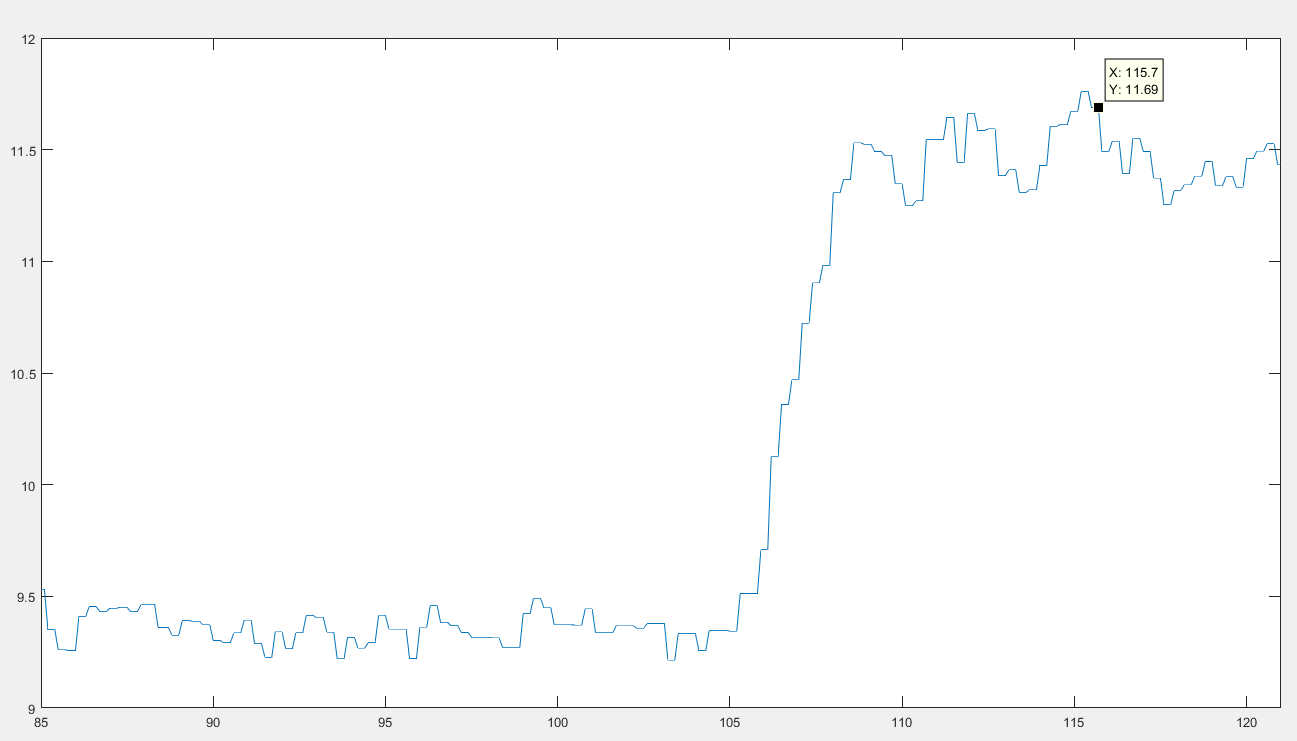
\includegraphics[width=0.9\linewidth]{Caudal_Max.png}
	\captionof{figure}{Máximo caudal}
	\label{fig:CM}
\end{figure}




\begin{comment}
\fcolorbox{red}{yellow}{Estuve viendo las curvas con escalones donde se ve que la ganancia estática se modifica frente a diferentes escalones. Si el objetivo fuese calcular un controlador para ese sistema una buena opción seria un controlador PI. De esta forma, la acción integral va a tratar de hacer que el error de estado estacionario sea cero frente a una entrada escalón. Además, los problemas que pueden existir en el envejecimiento de componentes, errores en el modelado y variaciones en la ganancia estática se van a mitigar con la parte integral del controlador. Obviamente al cambiar la planta la respuesta va a cambiar pero se va a cumplir la consigna de seguir la referencia. Para mostrar esto es posible calcular un controlador para un sistema y luego probar el controlador en los dos sistemas. Eso hice en el pdf que les adjunto con un sistema con 3 polos reales. Más detalles pueden encontrar en el libro de Ogata o Control avanzado de Karl Astrom, capitulo 3.
De esta forma, me da la sensación que para los objetivos de esta materia plantear un controlador PI para un controlador me parece bien.}
\end{comment}



